\documentclass[14pt,a4paper]{report}
\usepackage[utf8]{inputenc}
%Idioma
\usepackage[spanish]{babel}
\spanishdecimal{.}
%Para expresiones matematicas
\usepackage{titlesec}
\usepackage{amsmath}
\usepackage{amsfonts}
\usepackage{amssymb}
\usepackage{amstext}
\usepackage{mathtools}
\usepackage{mathrsfs}
\usepackage{physics}
%Imagenes
\usepackage{graphicx}
\usepackage{color}
%Para dibujar
\usepackage{tikz}
\usetikzlibrary{arrows.meta}
\usetikzlibrary{decorations.markings}
\usetikzlibrary{babel,patterns,snakes}
\usetikzlibrary{shapes.callouts}
\usetikzlibrary{calc,patterns,angles,quotes}
\usetikzlibrary{shadings}
%Cajas con colores
\usepackage{tcolorbox}
\tcbuselibrary{theorems}
%Ejemplo de lo anterior
%\begin{equation}
% a x^2 + bx + c = 0 \rightarrow
%\tcboxmath[colback=magenta!25!white,colframe=magenta, title=Solución]
%{x = \frac{-b\pm\sqrt{b^2-4ac}}{2a}}  
%\end{equation}
%
%Estilo fancy
\usepackage{fancyhdr}
%Interlineado y margenes y poco mas
\usepackage{setspace}
\usepackage{parskip}
\usepackage{multicol}
\usepackage[left=2.5cm,right=2.5cm,top=2.5cm,bottom=2.5cm]{geometry}
%Empieza documento
\begin{document}
%Cajas comentadas 
\newcommand{\commentedbox}[2]{%
  \mbox{
    \begin{tabular}[t]{@{}c@{}}
    $\boxed{\displaystyle#1}$\\
    #2
    \end{tabular}%
  }%
}
%Definimos el estilo de las paginas
\pagestyle{fancy}
\lhead{\itshape Cursos  - MCD}
\rhead{Proyecto Individual - Parte 2}
\Large{Matemáticas - \textit{Redes Neuronales}}\\
\normalsize
Rodolfo Armando Jaramillo Ruiz\\
05 de Mayo de 2023\\
\section*{Redes Neuronales Convolucionales}

Las redes neuronales se usan para resolver una gran variedad de problemas, uno de estos es procesar imágenes. Este, sin embargo, es un trabajo que si se pretende realizar usando, por ejemplo, una red neuronal multicapa solamente, haciendo que la entrada sea un vector que contenga los valores de los pixeles, se volvería un trabajo muy pesado a nivel de procesamiento, y los resultados serían muy deficientes. Es por eso que se aborda con otro método, usando otras operaciones que han probado mejorar el rendimiento de las redes para realizar tareas de procesamiento de imágenes.

\subsection*{Preámbulo}

\subsubsection*{Imágenes como matrices}

Las imágenes se pueden trabajar como una matriz de dos dimensiones, donde cada celda representa una característica especial. Por ejemplo, se puede pensar en una imagen en blanco y negro, donde cada celda tiene un valor entre 0 y 1, entonces cada celda tendrá un color correspondiente a este valor. Entonces, la imagen se puede traducir a una matriz de valores entre 0 y 1. Por lo que, por ejemplo, una imagen de $28\times28$ pixeles tiene sería un vector de 784 valores entre 0 y 1.

\begin{figure}[h]
  \centering
  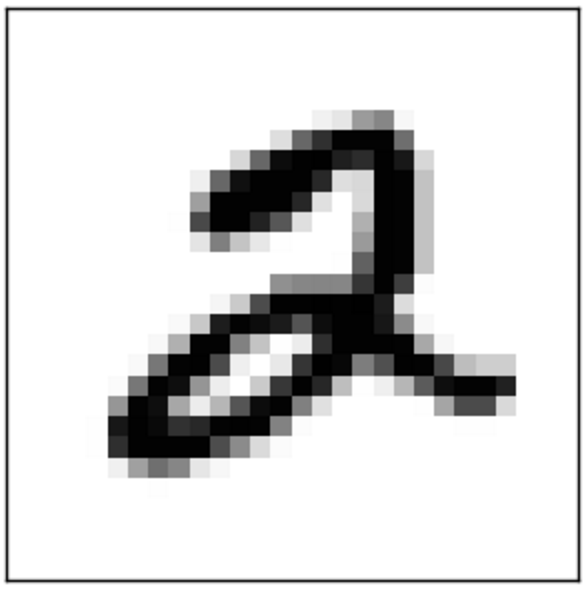
\includegraphics[scale=0.5]{../MNIST.png} 
  \caption{Numero manuscrito de la base de datos MNIST}
  \label{fig:neural-network}
\end{figure}

La figura 1 es una imagen en escala de grises que es equivalente a un vector de 784 valores que representan cada vector en una escala de grises.

Cuando se trabaja con imágenes con color, digamos, en el sistema RGB, se puede separar en tres imágenes; una que viene del canal rojo, otra que viene del canal verde, y otra que viene del canal azul. Entonces a cada imagen se le puede procesar de la misma forma como en el ejemplo anterior. Por lo que se tendría de una imagen, tres matrices del mismo tamaño que serían el \textit{input} de un solo ejemplo de la red neuronal en entrenamiento.

\subsubsection*{Redes neuronales multicapa}

Una red neuronal multicapa consta de una entrada y una salida, siendo la primera una serie de neuronas en forma de capa que reciben el \textit{input} en crudo, y la última otra serie de neuronas que indican el \textit{output} de la red. Además se tienen una cantidad no fija de capas intermedias cuyo \textit{input} es el \textit{output} de la capa anterior. Las conexiones entre capas pueden estar complemente conectadas o no, para el primer caso me referiré a ellas como \textit{full-conected}.

\subsection*{Operación de convolución}

Las redes neuronales se llaman así porque incluyen un tipo de capa especial donde se realiza una operación llamada convolución. Esta operación consiste en pasar la imagen por un filtro y generar una nueva imagen que provee información sobre la imagen original. Estas imágenes pasar por un filtro se llaman mapas de características. Las redes neuronales convolucionales pueden tener varias capas convolucion donde se extraen varios mapas de caracteristicas, antes de que se llegue a la parte de capas \textit{full-conected}

Este filtro, al que me referiré como kernel, es una matriz cuadrada con diferentes valores que definen el efecto que tiene el kernel sobre la imagen.

\begin{figure}[h]
  \centering
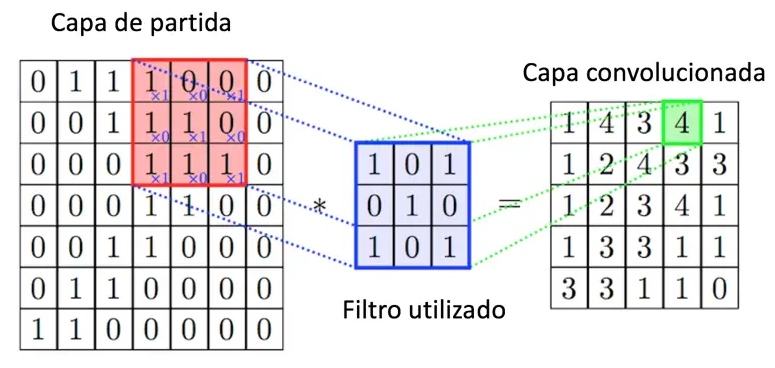
\includegraphics[scale=0.7]{../convolucion.png} 
  \caption{Operacion de convolución}
  \label{fig:neural-network}
\end{figure}

Lo que hace el kernel es convertir cada región de la imagen que cubre al superponerse sobre esta en una celda del mapa de características. La conversión se obtiene mediante la multiplicación punto por punto de los valores del kernel y los valores de la región que tiene el kernel superpuesto en este momento. Si se convierte el kernel y la región en dos vectores, la convolución sería hacer el producto punto entre ambos de la siguiente forma:
$$
\begin{bmatrix}
1 & 0 & 0 \\
1 & 1 & 0 \\
1 & 1 & 1 \\
\end{bmatrix}
*
\begin{bmatrix}
1 & 0 & 1 \\
0 & 1 & 0 \\
1 & 0 & 1 \\
\end{bmatrix}
=
4
$$
Es decir
$$
[1, 0, 0, 1, 1, 0, 1, 1, 1]\cdot[1, 0, 1, 0, 1, 0, 1, 0, 1]=4\\
$$

Así, se obtiene un mapa de  al pasar toda la imagen por este filtro. Como se puede ver, el mapa de  es una imagen de menores dimensiones que la imagen a la que se le aplicó el filtro. Esto no es un problema en sí mismo, pero se pueden hacer arreglos para que la imagen que salga del filtro sea de las mismas dimensiones. Eso se explicará en las siguiente sección.

Volviendo a las imágenes a color, al separarla en tres imágenes cómo se describió anteriormente, lo que se hace es obtener mapas de características, uno por cada canal de color.

En síntesis, la convolución es una operación que toma una imagen y la lleva a otro espacio, que podemos decirle espacio de características. El kernel de la convolución puede tener diferentes valores y formas, y se obtendrán diversos mapas que dan diversa información de las imágenes.

\subsection*{Otras operaciones básicas}
Hay un conjunto de operaciones asociadas a la convolución, aquí se muestran como un pequeño glosario:

El \textit{padding} es el medio por el cual se obtiene un mapa de caracteristicas el mismo tamaño que la imagen original. Esto se logra alterando dicha imagen para que ahora este rodeada por pixeles de valor cero, de modo que la aplicación del kernel se pueda realizar centrando el kernel incluso en los pixeles de la los bordes de la imagen, obtiene un pixel del mapa de características por cada pixel que existe en la imagen original.

El \textit{strides} hace referencia al desplazamiento que realiza el kernel a la hora de obtener el mapa. Este desplazamiento puede ser de una celda a la vez, que es lo tradicional, sin embargo puede ser mayor a uno. En combinación con el \textit{[padding} se pueden obtener más variedad de tamaño en los mapas de características, se obtiene una mayor libertad a la hora de obtener estos mapas.

El \textit{pooling} analiza el contenido de la imagen por bloques de celdas, es como aplicar una convolución en sí misma, la operación es muy similar. Esta operación permite reducir el número de datos mientras que la información se preserva. Lo que se hace es tomar una región minúscula de la misma forma que se hace al aplicar un fltro, y se ejecuta una operación entre las celdas para asignárselo a otro mapa de características, pero no ejecuta la convolución, si no alguna de las operaciones siguientes. Voy a nombrar dos tipos de pooling:\\
\begin{itemize}
\item \textit{Maxpooling}: se toma la región, se comparan los valores de las celdas para tomar el más grande.
\item \textit{Averagepooling}: se toma la región, y se devuelve el valor el promedio del valor de las celdas.
\end{itemize}

\begin{figure}[h]
  \centering
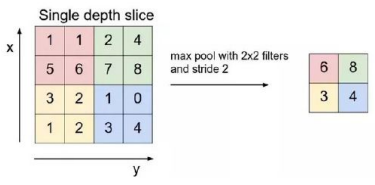
\includegraphics[scale=1]{../maxpooling.png} 
  \caption{Ejemplo de \textit{maxpooling} $2\times2$ con $\textit{stride}=2$}
  \label{fig:neural-network}
\end{figure}

El \textit{stacking} es el apilar el resultado de aplicarle a una imagen varios filtros para extraer la mayor cantidad de caracteristicas de una misma imagen. 

Por ejemplo, si a una imagen pequeña de $10 \times 10$ se le aplican 10 filtros de de $3 \times 3$. Considerando un \textit{padding} de 0, un \textit{stride} de 1, se obtiene una salida de volumen $8 \times 8 \times 10$, es decir, 10 mapas de caracteristicas de 64 pixeles cada uno.

Estos conceptos serán de ayuda para resolver el problema planteado en la primera parte del proyecto.

\subsection*{Problema}

El obtener paletas de colores es una tarea usual dentro del área del diseño y más oficios artísticos, así que me plantee como sería el funcionamiento de una red neuronal que reciba como \textit{input} una imagen y que el \textit{output} sea una paleta de colores. Para efectos prácticos, esta paleta será en forma de un vector de 10 colores, cada uno en forma de RGB. Se muestra un ejemplo de como sería la entrada esperada y la salida esperada.

\begin{figure}[h]
  \centering
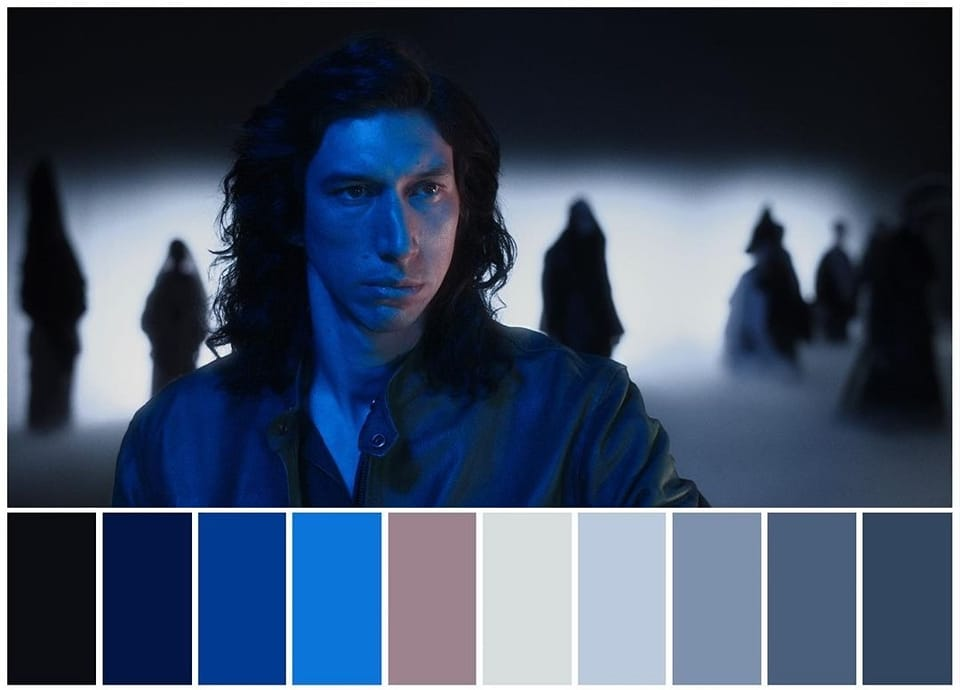
\includegraphics[scale=0.4]{../paleta-colores.jpg} 
  \caption{Frame de Annete (2021) - \textit{@CinemaPalettes} en \textit{Facebook}}
  \label{fig:neural-network}
\end{figure}

Este es un trabajo hecho completamente autor según el mismo autor. La idea es replicar estos resultados usando una red neuronal comvolucional.

\subsection*{Elección de metodología}

Existen varias formas abordar este problema, para este proyecto usaré una metodología usada en Prades [1]. Este a su vez, utilizó una arquitectura presentada en Wang [2]. Estos artículos abordan el procesamiento del color en imágenes para su etiquetado, por lo que su metodología encaja muy bien con el problema propuesto. Tomaré en cuenta las mismas consideraciones que se usaron en Prades [1], pero cuando estas dejen de ser apropiadas para este problema en particular lo señalaré y haré los cambios necesarios.

\subsection*{Arquitectura}

La arquitectura de la red consta de dos fases, cada una con un modelo diferente para obtener las características de las imágenes de entrada.

\textbf{Primera fase}: Se emplea un modelo de redes neuronales convolucionales (CNN) con el propósito de extraer características generales de las imágenes. El enfoque se centra en preservar y concentrar las características relacionadas con el color, sin la necesidad de utilizar etiquetas previas para clasificar los colores. Se propone el uso de un modelo de CNN auto-supervisado (SS-CNN) que se entrena mediante el uso de recortes aleatorios tomados de las imágenes del conjunto de entrenamiento. Los histogramas de color derivados de estos recortes se utilizan como una forma de supervisión interna para el entrenamiento del modelo.

\textbf{Segunda fase}: Consiste en afinar el modelo SS-CNN obtenido en la primera fase y reentrenar únicamente la última capa de la CNN utilizando imágenes etiquetadas con sus respectivos nombres de color. Sin embargo, es necesario abordar las muestras mal etiquetadas que pueden afectar el modelo resultante. Para ello, se aplica un proceso de refinamiento en el conjunto de entrenamiento para desechar las muestras que introducen ruido durante el entrenamiento de la CNN. El proceso de refinamiento implica predecir las etiquetas de los recortes de las imágenes de entrenamiento y seleccionar las muestras etiquetadas correctamente con la predicción más alta para cada color. Estas muestras seleccionadas se consideran "semillas" y se utiliza la tercera capa del modelo para calcular la media de estas semillas para cada uno de los 11 colores, estableciendo así un centro de clase para cada color. Luego, se descartan las muestras que se encuentran demasiado alejadas de los centros de clase establecidos. Una vez que se obtienen las muestras de entrenamiento "purificadas", se procede a otra fase de entrenamiento de la red utilizando estas muestras filtradas. Este proceso de selección de muestras y entrenamiento se repite N veces en el modelo.

\subsection*{Implementación en papel}

\subsubsection*{Generación de histogramas}
La primera fase del modelo es un SS-CNN. La función de los histogramas es que supervisen el entrenamiento de la red, ya que para cada imagen de entrenamiento describen la distribución de probabilidad de diferentes colores en cada una de las imagenes. Como la distribución de los colores en el espacio RGB es desigual no se puede hacer un histograma de la manera habitual. Para resolver este problema, se usará el algoritmo \textit{k-means} con el fin de clasificar el todos  los pixeles de una imagen en 128 \textit{clusters} representados en el espacio RGB.

\begin{figure}[h]
  \centering
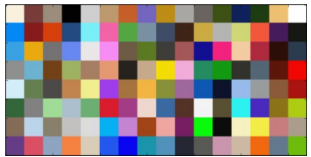
\includegraphics[scale=0.7]{../clusters-kmeans.png} 
  \caption{Los 128 \textit{clusters} en el espacio RGB}
  \label{fig:neural-network}
\end{figure}

El algoritmo de \textit{k-means} funciona tomando las $n$ observaciones, que para este caso serian los \textit{inputs} de la imagen, y asignandolos en los $k$ centroides iniciales $m_1, m_2, ... m_k$ en función de su distancia a este. Este algoritmo itera en dos pasos.
\begin{enumerate}
\item Asignación: usando notación de conjuntos, para un grupo $S^{(t)}_{i}$ (donde $t$ indica a que iteración corresponde este centroide) le corresponden los siguientes elementos según la ecuación.

$$
S^{(t)}_{i} = \{x_p:||x_p-m^{(t)}_{i}||\leq||x_p-m^{(t)}_{j}||\forall 1\leq j \leq k\}
$$
Es decir, a cada grupo se le asignan los elementos que estén más cerca de su centroide respectivo.
\item Actualización: Los centroides van cambiando en cada iteración según la siguiente expresión:

$$
m^{(t+1)}_{i} = \frac{1}{|S^{(t)}_{i}|}\sum_{x_{j}}\in S^{(t)}_{i}x_{j}
$$

Es decir, se calcula el centroide de los elementos que están asignados en un grupo, y este se vuelve el nuevo centroide.

\end{enumerate} 

Entonces, \textit{k-means} asigna a las observaciones en grupos, pero no necesariamente el centroide de los asignados coincide, por lo que se calcula este último para cambiarlo. Se vuelve a hacer la asignación con los nuevos centroides hasta que el proceso converga, que será cuando las asignaciones no cambien.

Los \textit{clusters} obtenidos con este algoritmo son los que se usan para construir con los histogramas de las imágenes. A cada pixel se le asignará se le asignará su representante más cercano en el espacio RGB.

Para cada imagen se obtiene un vector de 128 elementos, donde cada uno representa la cantidad de pixeles de esa imagen que se acercan más al color que corresponde esa posición. Al normalizar, se obtiene un vector de probabilidades, donde la suma de todos los elementos da como resultado la unidad.

\subsubsection{Implementación del modelo SS-CNN}

El modelo consiste en 3 capas convolucionales y una capa final que será \textit{full-conected}. La primera convolución consta de 32 nodos, las siguientes dos serán de 96 nodos, mientras que la última capa será de 128 nodos. Pero también, entre cada capas intermedias. La función de estas capas se enlista a continuación:
\begin{itemize}
\item \textit{Rectifer Linear Units}: (ReLU) Se trata de implementar una función de activación de la forma $f(v_k) = max(0, v_k)$ para aumentar las propiedades no lineales de la función de decisión.

\begin{figure}[h]
  \centering
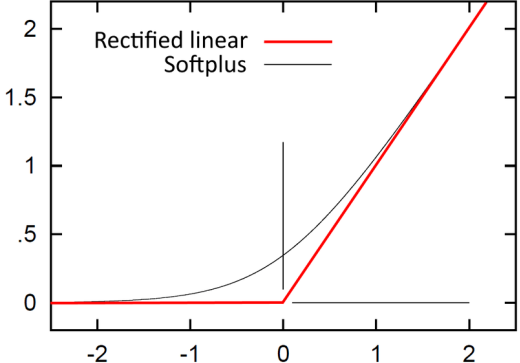
\includegraphics[scale=0.6]{../relu.png} 
  \caption{Gráfica de la función ReLU}
  \label{fig:neural-network}
\end{figure}

\item \textit{Maxpooling} Se realiza esta operación para reducir el tamaño de la salidas.
\item \textit{Local response normalization}: (LRN) Para normalizar las salidas de ReLU, porque las salidas de suelen tener valores en un rango arbitrario.
\end{itemize}

La primera y segunda convolución son seguidas por capas ReLU, \textit{maxpooling} y LRN, la tercera no tiene LRN. Además, los kernels son de tamaño $3\times3$, mientras que los \textit{strides} son de 1 para las primeras dos convoluciones, y de 2 para la tercera. Se utilizaran recortes de las imágenes de entrenamiento de tamaño de $37\times 37$ pixeles.

\begin{figure}[h]
  \centering
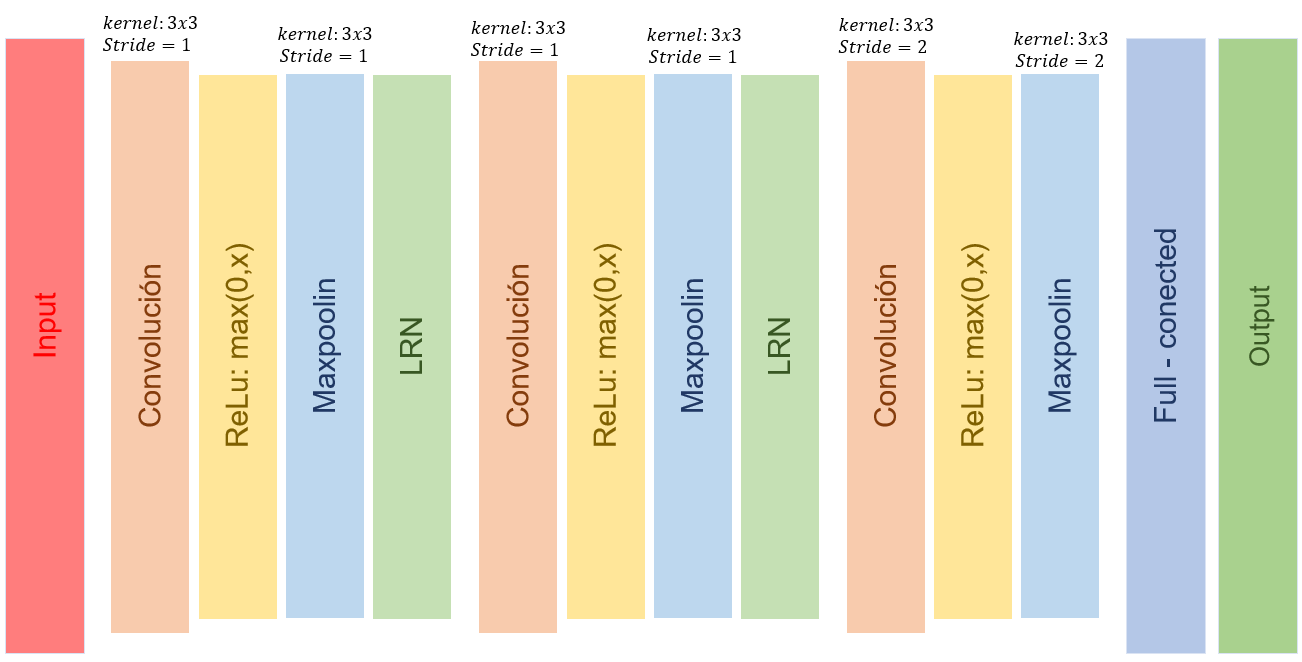
\includegraphics[scale=0.5]{../esquema-capas.png} 
  \caption{Esquema de las capas de SS-CNN}
  \label{fig:neural-network}
\end{figure}

Para entrenar a la red se hará \textit{backpropagation} usando descenso de gradiente. Para esto, usaré la función de perdida de \textit{cross entropy}:

$$
\varepsilon = -\frac{1}{n}\sum^{n}_{i=1}\sum^{c}_{j=1}\hat{p}_{ij}log(p_{ij})
$$

Detallando la expresión anterior, $n$ es la cantidad de ejemplos de entrenamientos. En este caso, imagenes. Mientras que $c$ es la cantidad de clasificaciones posibles, que son 128 siempre, por la forma en que se crearon los histogramas. Los valores $p_{ij}$ y $\hat{p}_{ij}$ son la probabilidad de que la imagen $i$ pertencezca a la clase $j$, solo que la primera es la probabilidad dada por la red, mientras que la segunda es la probabilidad dada por el vector de supervisión, que corresponde al vector de probabilidad obtenido en el histograma.

A partir del modelo inicial de SS-CNN, se realiza un proceso de refinamiento conocido como \textit{finetuning}. Durante este proceso, la última capa se reentrena utilizando las mismas imágenes de entrenamiento utilizadas anteriormente. En el \textit{finetuning}, todas las capas del modelo se mantienen fijas, y solo la última capa completamente conectada se reentrena siguiendo las estructuras clásicas de los modelos CNN. Sin embargo, la salida de la última capa se modifica para adaptar el modelo a la clasificación de colores en 11 categorías distintas basadas en la clasificación propuesta por Berlin y Kay.

El nuevo modelo resultante se verá claramente afectado por las imágenes mal etiquetadas y estará lejos de ser preciso. Las imágenes utilizadas para el entrenamiento del modelo tienen etiquetas globales, pero en muchos casos, el color solo se encuentra en una pequeña región de la imagen o se corresponde con un objeto específico en presencia de otros colores en la imagen. Incluso hay casos en los que las etiquetas de las imágenes están completamente equivocadas, llegando al extremo de que una imagen etiquetada con un color no contenga ni un solo pixel de ese color.

Por lo tanto, se aplica un proceso de selección de muestras en los pasos siguientes, con el fin de descartar las muestras etiquetadas erróneamente y obtener un conjunto de muestras "purificadas" que se utilizarán para reentrenar el modelo.

\newpage
\section*{Bibliografía}
\begin{enumerate}
\item O. Prades “\textit{Descripcion de los colores de una imagen mediante tecnicas de Deep learning}”, Escola D’enginyeria, Universotat Autómata de Barcelona, Barcelona, España, 2017

\item Y. Wang, J. Liu, J. Wang, Y. Li, H. Lu, “\textit{Color names learning using convolutional neural networks}”, The National Laboratory of Pattern Recognition, Institute of Automation, Chinese Academy of Sciences, Beijing, China, 2015
\end{enumerate}



\end{document}